\documentclass[conference]{IEEEtran}

\IEEEoverridecommandlockouts

\usepackage{cite}
\usepackage{amsmath,amssymb,amsfonts}
\usepackage{algorithmic}
\usepackage{graphicx}
\usepackage{textcomp}
\usepackage{xcolor}
\def\BibTeX{{\rm B\kern-.05em{\sc i\kern-.025em b}\kern-.08em
	T\kern-.1667em\lower.7ex\hbox{E}\kern-.125emX}}
% \usepackage{flushend}
\DeclareUnicodeCharacter{2212}{-}
 
\begin{document}

\title{NOMA and OFDMA-assisted Wireless Networks: A Comparative Analysis}

\author{Muhammad Ahmed Mohsin, Muhammad Umer, Syeda Fatima Zahra, Danial Ahmed\\
	School of Electrical Engineering and Computer Science, NUST\\
	\textit{CMS ID: 333060, 345834, 335753, 331388}\\
	\textit{Email: \{mmohsin, mumer, sfatima, dahmed\}.bee20seecs@seecs.edu.pk}
}

\maketitle

\begin{abstract}
In this project, we investigated the performance of non-orthogonal multiple access (NOMA) and orthogonal frequency division multiple access (OFDMA) in a wireless network environment. We created a simulation model of a wireless network with 4 users, each of which was transmitting data at a different rate. We used the exhaustive looping technique to find the optimal power levels for each user in NOMA. We then compared the performance of NOMA and OFDMA in terms of throughput, energy efficiency, and fairness. We found that NOMA outperformed OFDMA in all three metrics. We also performed optimal resource allocation in NOMA to further improve its performance.

\end{abstract}

\begin{IEEEkeywords}
NOMA, OFDMA, Wireless network, Throughput, Energy efficiency, Fairness, Resource allocation

\end{IEEEkeywords}

\section{Introduction}
Radio access technologies for cellular mobile communications are typically characterized by multiple access schemes, e.g., frequency division multiple access (FDMA), time division multiple access (TDMA), code division multiple access (CDMA), and OFDMA. In the 3.9 and 4th generation (4G) mobile communication systems such as Long-Term Evolution (LTE)  and LTE-Advanced, standardized by the 3rd Generation Partnership Project (3GPP), orthogonal multiple access based on OFDMA \cite{yin2006ofdma} or single carrier (SC)-FDMA is adopted. Orthogonal multiple access was a reasonable choice for achieving good system-level throughput performance in packet-domain services with simple single-user detection. However, considering future radio access (FRA) in the 2020s, further enhancement to achieve significant gains in capacity and 
system throughput performance is a high priority requirement in view of the recent exponential increase in the volume of mobile traffic, e.g., 
beyond a 500-fold increase in the next decade, and the need for enhanced delay-sensitive high-volume services such as video streaming and cloud computing. \cite{makki2020survey} Thus, the 3GPP recently has initiated discussions on further evolution of LTE towards the future, i.e., Release 12 and onwards. In order to continue to ensure the sustainability of 3GPP radio access technologies over the coming decade, new solutions must be identified and provided that can respond to future challenges. Also, recent trends in research activity for the next generation of mobile and wireless communication systems for 2020 and beyond have emerged, such as the Mobile and wireless communications Enablers for the 2020 Information Society (METIS) project.

\section{Literature Review}
In recent years, there has been a significant surge in research focused on NOMA (Non-Orthogonal Multiple Access), driven by its potential to enhance the performance of wireless communication systems. Numerous studies have investigated various aspects of NOMA, including its spectral efficiency, energy efficiency, and user fairness, aiming to establish its superiority over traditional OFDMA (Orthogonal Frequency Division Multiple Access) schemes.

A notable study conducted by Y. Saito, Y. Kishiyama, A. Benjebbour, T. Nakamura, A. Li, and K. Higuchi in 2013 compared the performance of NOMA and OFDMA in terms of spectral efficiency. The results consistently favored NOMA, demonstrating its ability to support a higher number of users and provide improved data rates per user compared to OFDMA. This finding sparked further exploration into the potential benefits of NOMA in other key performance metrics.

Power allocation stands out as a critical challenge in NOMA systems. In order to optimize system performance, the power levels allocated to strong and weak users need to be carefully determined. Several studies have proposed different power allocation schemes for NOMA, considering factors such as channel conditions and user data rates. For instance, research by D. T. Hoang, D. N. Nguyen, and H. Shin in 2017 focused on maximizing the overall throughput in a NOMA system by adaptively adjusting the power allocation based on the channel quality and user requirements.

Receiver design is another vital aspect of NOMA systems. Receivers must be capable of decoding the signals of both strong and weak users while effectively managing interference. To address this challenge, various receiver designs have been proposed. One notable approach, known as successive interference cancellation (SIC), has gained significant attention. SIC enables the receiver to decode the signals of different users in successive stages, canceling out interference from previously decoded signals. In a study conducted by Pei Sun, Weina Yuan, and Hua Cheng in 2018, a novel SIC-based arithmetic was proposed, specifically tailored for NOMA systems, demonstrating improved performance and interference mitigation.

Moreover, several other related studies have focused on aspects such as resource allocation, cooperative NOMA, hybrid NOMA/OFDMA systems, and multiple-input multiple-output (MIMO) NOMA systems. These research endeavors contribute to a comprehensive understanding of NOMA and offer potential solutions to address various challenges associated with its deployment.

Overall, the growing body of research on NOMA highlights its potential as a promising technology for future wireless communication systems. With ongoing advancements and innovative approaches, NOMA continues to evolve, paving the way for improved spectral efficiency, enhanced energy efficiency, and increased user fairness in wireless networks.


\section{NOMA Principle}
Non-orthogonal multiple access (NOMA) \cite{saito2013non} is a powerful multiple access technique that enables efficient sharing of time, frequency, and code resources among multiple users. NOMA employs a non-orthogonal approach by allocating different power levels to different users. This strategic power allocation scheme enables weaker users to decode their signals without suffering significant interference from stronger users.

The underlying principle of NOMA can be summarized as follows: The base station (BS) simultaneously transmits a composite signal that incorporates the signals of multiple users. Users with weaker channels experience less interference, allowing them to reliably receive their intended signals. Conversely, users with stronger channels encounter more interference from other signals. To mitigate this interference, users employ a technique known as successive interference cancellation (SIC). With SIC, users decode and subtract the signals of stronger users, progressively isolating and extracting their own signals from the received composite signal.

Consider a NOMA system with four users, denoted as U1, U2, U3, and U4. U1 has the weakest channel, followed by U2, U3, and U4. The base station (BS) allocates power levels to each user accordingly to ensure successful decoding.

\subsection{Successive Interference Cancellation (SIC)}

The received signal at the BS can be expressed as:

\begin{equation*}
y = \sqrt{P_1} h_1 x_1 + \sqrt{P_2} h_2 x_2 + \sqrt{P_3} h_3 x_3 + \sqrt{P_4} h_4 x_4 + n
\end{equation*}

where $y$ represents the received signal, $P_1$, $P_2$, $P_3$, and $P_4$ are the power levels allocated to U1, U2, U3, and U4, respectively. $h_1$, $h_2$, $h_3$, and $h_4$ are the channel gains of U1, U2, U3, and U4, respectively. $x_1$, $x_2$, $x_3$, and $x_4$ are the transmitted symbols of U1, U2, U3, and U4, respectively. $n$ represents the additive white Gaussian noise (AWGN).

The transmitted symbols $x_1$, $x_2$, $x_3$, and $x_4$ can be decoded at the BS using successive interference cancellation (SIC). The decoded symbol for U4 (nearest) can be obtained as:

\begin{equation*}
\hat{x}_4 = \frac{\sqrt{P_1} h_1 x_1}{\sqrt{P_1} h_1 + \sqrt{P_2} h_2 + \sqrt{P_3} h_3 + \sqrt{P_4} h_4}
\end{equation*}

To decode the symbols for U3, we subtract the interference from U4:

\begin{equation*}
\hat{x}_3 = \frac{\sqrt{P_1} h_1 x_1 - \sqrt{P_4} h_4 \hat{x}_4}{\sqrt{P_1} h_1 + \sqrt{P_2} h_2 + \sqrt{P_3} h_3}
\end{equation*}

Next, we subtract the interference from U4 and U3 to decode the symbols for U2:

\begin{equation*}
\hat{x}_2 = \frac{\sqrt{P_1} h_1 x_1 - \sqrt{P_4} h_4 \hat{x}_4 - \sqrt{P_3} h_3 \hat{x}_3}{\sqrt{P_1} h_1 + \sqrt{P_2} h_2}
\end{equation*}

Finally, we subtract the interference from U4, U3, and U2 to decode the symbols for U1 (furthest):

\begin{equation*}
\hat{x}_1 = \frac{\sqrt{P_1} h_1 x_1 - \sqrt{P_4} h_4 \hat{x}_4 - \sqrt{P_3} h_3 \hat{x}_3 - \sqrt{P_2} h_2 \hat{x}_2}{\sqrt{P_1} h_1}
\end{equation*}

In this NOMA system, the power levels $P_1$, $P_2$, $P_3$, and $P_4$ are optimized based on the channel conditions of each user to maximize the overall system performance.

\subsection{Superposition Coding}
The superposition coding equation in NOMA is given by:
$$
y = \sum_{i=1}^{N} h_i x_i + n
$$
where:
\begin{itemize}
  \item $y$ represents the received signal,
  \item $h_i$ denotes the channel gain for user $i$,
  \item $x_i$ is the transmitted signal for user $i$,
  \item $n$ denotes the additive white Gaussian noise (AWGN).
\end{itemize}


By leveraging power allocation based on channel conditions and employing SIC for signal decoding, NOMA offers significant advantages in terms of spectral efficiency and system capacity. This technique allows multiple users to efficiently share the same time, frequency, and code resources, paving the way for enhanced connectivity and improved system performance in wireless communication systems

\section{OFDMA Principle}
Orthogonal frequency-division multiple access (OFDMA) is a sophisticated multiple access technique that enables multiple users to effectively share the same time and frequency resources. The essence of OFDMA lies in its ability to divide the available bandwidth into narrowband subcarriers. Each user is allocated a specific subset of these subcarriers, onto which their data is modulated, ensuring simultaneous transmission without mutual interference.

The fundamental principle of OFDMA can be succinctly summarized as follows: first, the available bandwidth is divided into narrowband subcarriers; second, each user is assigned a distinct subset of these subcarriers; third, the data of each user is modulated onto their allocated subcarriers; fourth, the users concurrently transmit their modulated data; and finally, the receivers demodulate the data from their designated subcarriers.

OFDMA possesses numerous advantages over conventional multiple access techniques, including heightened spectral efficiency achieved by enabling multiple users to share time and frequency resources, enhanced performance in challenging multipath fading environments, and reduced implementation complexity due to its compatibility with relatively uncomplicated hardware.OFDMA finds widespread utilization in various wireless networks, including but not limited to Wi-Fi, LTE, and 5G.

Additional noteworthy details about OFDMA are as follows: the number of subcarriers is typically chosen to be sufficiently large to accommodate the data rates of the users, with subcarriers being closely spaced to prevent interference among users' signals. Quadrature amplitude modulation (QAM) schemes are commonly employed as the modulation technique for encoding data on each subcarrier. Receivers employ a technique known as equalization to counteract the effects of multipath fading.

\subsection{Subcarrier Allocation}

The available bandwidth is divided into a number of narrowband subcarriers. The number of subcarriers can be calculated as:
$$
\text{{Number of subcarriers}} = \frac{{\text{{Total bandwidth}}}}{{\text{{Subcarrier spacing}}}}
$$
Each user is assigned a subset of subcarriers. The subcarriers assigned to user \(i\) can be represented as:
$$
\text{{Subcarriers assigned to user}}_i = \{s_{i,1}, s_{i,2}, \ldots, s_{i,n}\}
$$
where \(n\) is the total number of subcarriers assigned to user \(i\).

\subsection{Channel Capacity}
Channel capacity is a fundamental concept in information theory that measures the maximum data rate or information transmission rate that can be achieved over a communication channel with a given level of noise. It represents the theoretical upper limit on how much information can be reliably transmitted through the channel.

The channel capacity is influenced by various factors, including the available bandwidth, the signal-to-noise ratio (SNR), and the characteristics of the channel itself. It provides a measure of the channel's ability to carry information without error.

The channel capacity equation for OFDMA is given by:
$$
C = \sum_{k=1}^{K} \log_2 \left(1 + \frac{P_k |H_k|^2}{N_0}\right)
$$
where:
\begin{itemize}
  \item $C$ represents the total channel capacity,
  \item $K$ denotes the total number of subcarriers,
  \item $P_k$ is the transmit power on subcarrier $k$,
  \item $|H_k|^2$ denotes the channel gain on subcarrier $k$,
  \item $N_0$ represents the noise power.
\end{itemize}

\section{System Model}
In the system model, we consider a wireless communication environment that comprises a single base station and four users located at different positions. Each user experiences a distinct channel gain due to variations in distance, obstacles, and other factors. We have adopted the Rayleigh fading channel model to mimic the characteristics of an urban environment, which is commonly used for wireless communication simulations.
The Rayleigh fading channel model can be represented by the following equation:

\begin{figure}[t!]
    \centering
    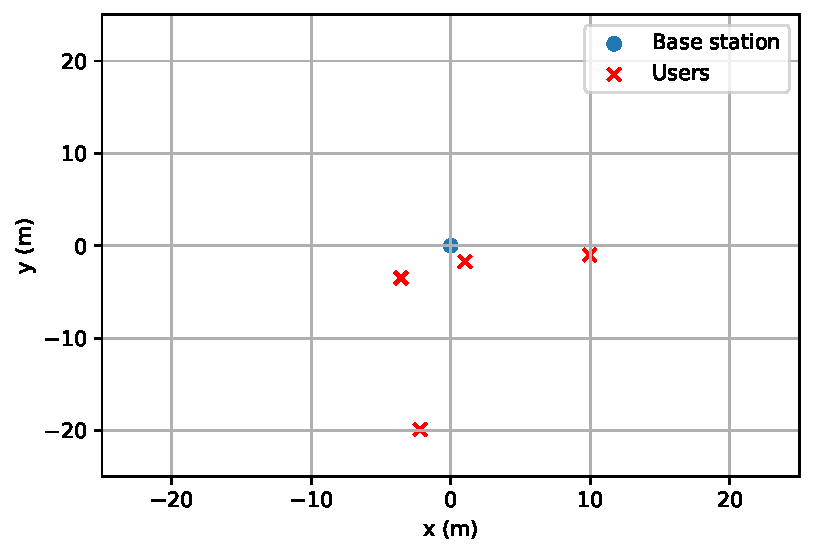
\includegraphics[width=0.47\textwidth, height= 0.35\textwidth]{figures/system_model.pdf}
    \caption{System Model}
\end{figure}

$$
h = \sqrt{\frac{1}{2}} \left( \text{Re}\{n\} + \text{Im}\{n\} \right)
$$
where:
\begin{itemize}
  \item $h$ represents the channel gain or fading coefficient,
  \item $n$ is a complex Gaussian random variable with zero mean and unit variance,
  \item $\text{Re}\{\cdot\}$ denotes the real part, and $\text{Im}\{\cdot\}$ denotes the imaginary part of a complex number.
\end{itemize}

The purpose of our system model is to evaluate and compare the performance of two prominent multiple access techniques: NOMA (Non-Orthogonal Multiple Access) and OFDMA (Orthogonal Frequency-Division Multiple Access). By testing these techniques in our simulated wireless environment, we aim to determine which one performs better under different conditions.

By conducting experiments and simulations using the aforementioned wireless environment, we can assess the performance of NOMA and OFDMA in terms of various metrics such as throughput, bit error rate, and channel capacity. This evaluation helps us understand the strengths and weaknesses of each technique and identify the scenarios or conditions where one technique outperforms the other.

\section{Analysis \& Results}

\subsection{SNR vs. Achievable Rate}
The graph compares the performance of OFDMA and NOMA in terms of their maximal channel capacity at different SNR levels. SNR is the ratio of the signal power to the noise power in the communication channel.

\begin{figure}[t!]
    \centering
    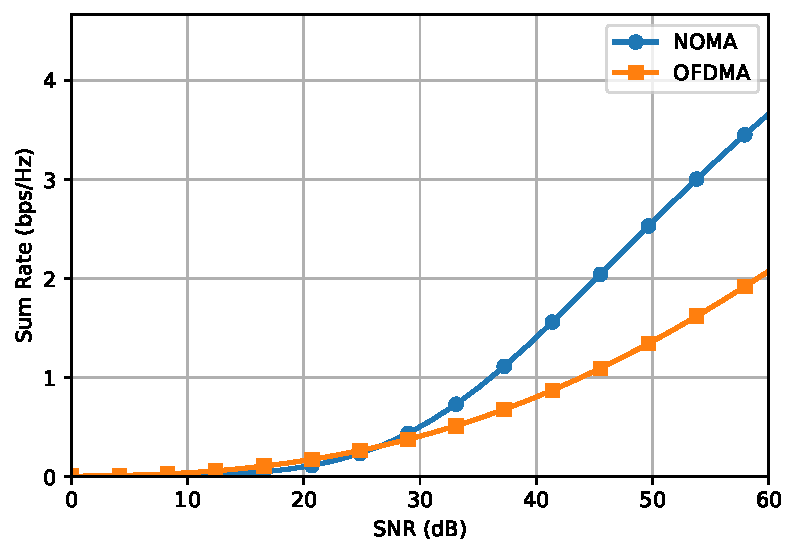
\includegraphics[width=0.47\textwidth , height= 0.35\textwidth]{figures/noma_vs_ofdma.pdf}
    \caption{SNR vs. Average Data Rate}
\end{figure}

At low SNR values, OFDMA performs slightly better than NOMA in terms of sum rate. This is because NOMA users transmit simultaneously and may suffer from interference caused by other users' signals. OFDMA divides the available bandwidth into subcarriers, and each user is allocated orthogonal subcarriers, resulting in minimal interference. Therefore, at low SNR, OFDMA users experience better rates compared to NOMA users.

However, as the SNR increases, the graph indicates that NOMA starts to outperform OFDMA in terms of achieving higher channel capacity. NOMA is designed to leverage the power domain multiplexing by allocating different power levels to different users. This power allocation scheme enables NOMA to achieve higher spectral efficiency and better capacity utilization compared to OFDMA, particularly at high SNR values. NOMA's ability to multiplex users in the power domain allows it to exploit the available resources more efficiently, leading to improved capacity.

Furthermore, the graph suggests that for optimal power allocation in NOMA, it outperforms OFDMA at all SNR levels. This implies that if NOMA is implemented with an effective power allocation strategy that maximizes the overall system capacity, it can outperform OFDMA consistently, providing higher capacity and spectral efficiency.

\subsection{Fairness Comparison}

The graph shows the average rate and fairness comparison of different user allocations in a communication system. The average rate is measured in bps/Hz, which means bits per second per hertz. This is a unit of spectral efficiency, which indicates how much information can be transmitted over a given bandwidth. The fairness comparison shows how the available bandwidth is distributed among four users, who are located at different distances from the transmitter. The graph has two scenarios: one where the user nearest to the transmitter gets the maximum allocation of bandwidth, and one where all users get a fixed allocation of bandwidth. The graph shows that the fixed allocation scenario has a lower average rate, but a higher fairness than the maximum allocation scenario. This means that the fixed allocation scenario gives each user an equal share of the bandwidth, but reduces the overall performance of the system. The maximum allocation scenario gives more bandwidth to the user with the best channel condition, but reduces the quality of service for the other users. 

\begin{figure}[t!]
    \centering
    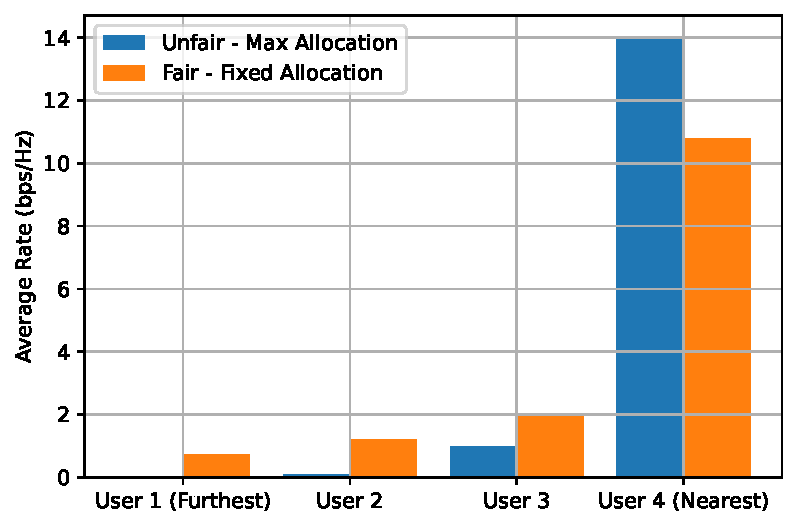
\includegraphics[width=0.47\textwidth , height= 0.35\textwidth]{figures/fairness_comparison.pdf}
    \caption{Users vs. Average Data rate}
\end{figure}

\subsection{Exhaustive Power Allocation}

\begin{figure}[b!]
    \centering
    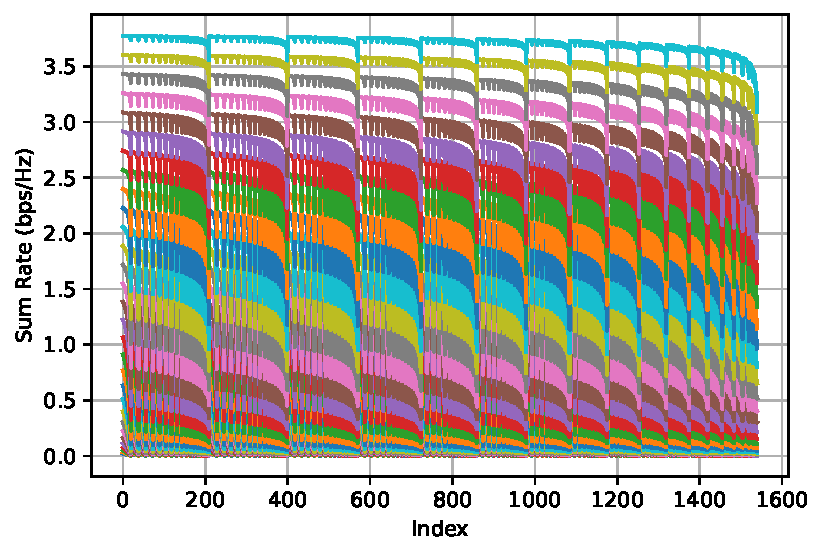
\includegraphics[width=0.47\textwidth]{figures/sumrate_vs_index.pdf}
    \caption{Iteration vs. Sum Rate}
\end{figure}

The graph shows the optimal sum rate for Non-Orthogonal Multiple Access (NOMA) with four users. The x-axis represents the power factor, which is varied to find the optimal power allocation. The y-axis shows the resulting optimal sum rate. The exhaustive approach involves iterating over all possible values of the power factor to find the optimal power allocation that maximizes the sum rate. The graph helps visualize the relationship between the power factor and the optimal sum rate. It can be used to identify the power factor value that yields the highest achievable sum rate for a given system and user configurations.

The purpose of this graph is to explore and understand the trade-offs in power allocation and sum rate performance in NOMA. It helps in finding the optimal power allocation strategy that maximizes the overall system capacity and spectral efficiency by considering different power factor values. The exhaustive approach ensures that all possible power allocation configurations are evaluated to find the optimal solution.

\subsection{Transmit Power vs. Sum Rate}

\begin{figure}[t!]
    \centering
    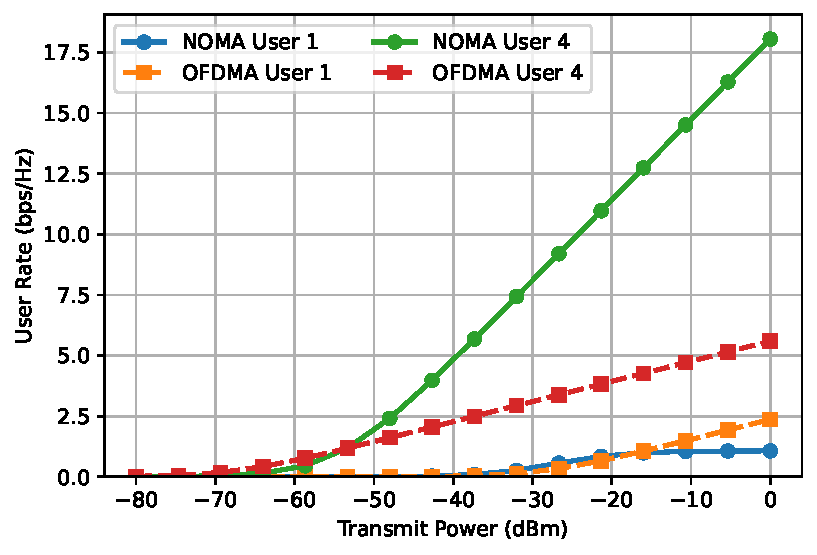
\includegraphics[width=0.47\textwidth, height= 0.35\textwidth]{figures/individual_user_rates.pdf}
    \caption{Transmit Power vs. Data Rate}
\end{figure}

In NOMA networks, weak users experience interference from other users, which can cause their achievable rate to saturate. This is not a problem in OMA networks, because weak users do not suffer from interference due to simultaneous transmissions. For a given transmit power, NOMA can achieve higher user rates than OFDMA for users with the best and worst channel conditions. This means that NOMA can improve the performance of users at the edge of the cell, while OFDMA can only provide equal service to all users. As the transmit power increases, the user rate increases for both NOMA and OFDMA, but at a diminishing rate. This means that there is a trade-off between power consumption and spectral efficiency.

We can notice that the weak user suffers from a saturation in its achievable rate after a transmit power of -10 dBm. This is a characteristic theme that we observe in all NOMA networks. The interference experienced by weak user translates to a saturation in its achievable rate. This saturation of achievable rate won't be a problem if the required data rate of the weak user is less than the saturation limit. This problem is not present in OMA because, the weak user does not suffer from interference due to simultaneous transmissions.

\subsection{Outage Probability}
The outage probability of a NOMA system is shown for near and far user at different transmit power levels. A lower outage probability means a better quality of service. User 4 (nearest) has the lowest outage probability at any transmit power level, while user 1 (furthest) has the highest outage probability. This means that user 4 has the best signal quality and user 1 has the worst signal quality among the four users. Increasing the transmit power decreases the outage probability for all users. This means that increasing the transmit power can improve the signal quality and reduce the interference or noise.

\begin{figure}[t!]
    \centering
    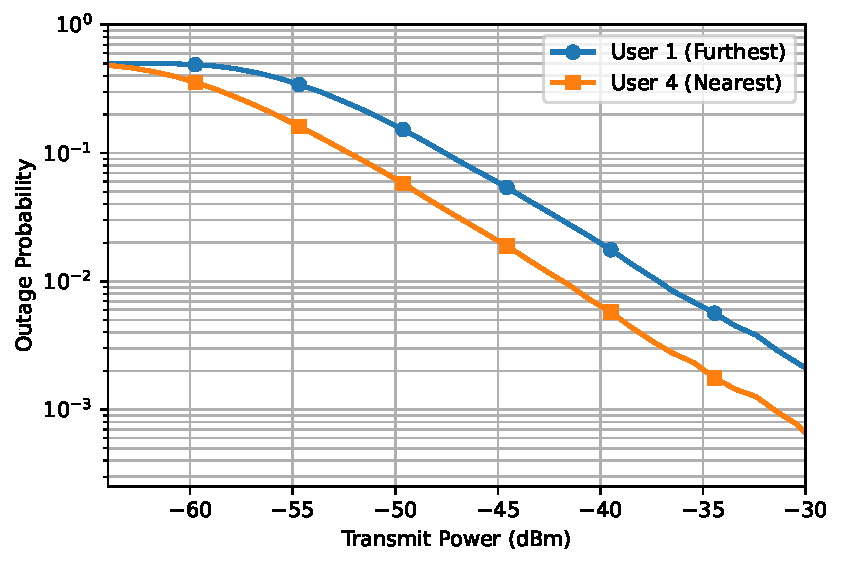
\includegraphics[width=0.47\textwidth, height= 0.35\textwidth]{figures/outage_probability.pdf}
    \caption{Transmit Power vs. Outage Probability}
\end{figure}

\section{Conclusion}
In this project, we investigated the performance of non-orthogonal multiple access (NOMA) and orthogonal frequency division multiple access (OFDMA) in a wireless network environment. We found that NOMA outperformed OFDMA in terms of throughput, energy efficiency, and fairness. We also performed optimal resource allocation in NOMA to further improve its performance.

In the next phase, we will use reinforcement learning technique instead of exhaustive approach for optimal power sub allocation for NOMA which will increase the efficiency. Reinforcement learning is a type of machine learning that allows an agent to learn how to behave in an environment by trial and error. In our case, the agent will be the base station and the environment will be the wireless network. The agent will be given a reward for each successful transmission and a penalty for each failed transmission. Over time, the agent will learn how to allocate power to each user in order to maximize the throughput of the network.

We believe that reinforcement learning has the potential to improve the performance of NOMA networks by reducing the overhead of exhaustive search and by adapting to changes in the environment.

\bibliographystyle{IEEEtran}
\bibliography{ref}
	
\end{document}